%
% File acl2021.tex
%
%% Based on the style files for EMNLP 2020, which were
%% Based on the style files for ACL 2020, which were
%% Based on the style files for ACL 2018, NAACL 2018/19, which were
%% Based on the style files for ACL-2015, with some improvements
%%  taken from the NAACL-2016 style
%% Based on the style files for ACL-2014, which were, in turn,
%% based on ACL-2013, ACL-2012, ACL-2011, ACL-2010, ACL-IJCNLP-2009,
%% EACL-2009, IJCNLP-2008...
%% Based on the style files for EACL 2006 by 
%%e.agirre@ehu.es or Sergi.Balari@uab.es
%% and that of ACL 08 by Joakim Nivre and Noah Smith
\pdfoutput=1
\documentclass[11pt,a4paper]{article}
\usepackage[hyperref]{acl2021}
\usepackage{times}
\usepackage{latexsym}
\usepackage{amsmath}
\usepackage{multirow}
\usepackage{booktabs}
\usepackage{graphicx}
\usepackage{amsfonts}
% \usepackage[demo]{graphicx}
\usepackage{subcaption}
\renewcommand{\UrlFont}{\ttfamily\small}

% This is not strictly necessary, and may be commented out,
% but it will improve the layout of the manuscript,
% and will typically save some space.
\usepackage{microtype}

\aclfinalcopy % Uncomment this line for the final submission
\def\aclpaperid{527} %  Enter the acl Paper ID here

%\setlength\titlebox{5cm}
% You can expand the titlebox if you need extra space
% to show all the authors. Please do not make the titlebox
% smaller than 5cm (the original size); we will check this
% in the camera-ready version and ask you to change it back.

\newcommand\BibTeX{B\textsc{ib}\TeX}

\title{Out-of-Scope Intent Detection with Self-Supervision and\\ Discriminative Training}

\author{
Li-Ming Zhan$^1$ \quad Haowen Liang$^1$\thanks{~ Equal contribution.}  \quad Bo Liu$^{1*}$ \quad Lu Fan$^1$ \quad Xiao-Ming Wu$^1$\Thanks{~ Corresponding author.} \\
\quad \bf Albert Y.S. Lam$^2$ \\ 
% {\bf \quad Xiao-Ming Wu$^1$\Thanks{~ Corresponding author.} \quad Albert Y.S. Lam$^2$} \\
Department of Computing, The Hong Kong Polytechnic University, Hong Kong S.A.R.$^1$ \\
Fano Labs, Hong Kong S.A.R.$^2$ \\
{\tt \{lmzhan.zhan, michael.liang, doc-bo.liu\}@connect.polyu.edu.hk}\\
% {\tt \{newmichael852,boliu.kelvin\}@gmail.com}\\
{\tt \{cslfan, csxmwu\}@comp.polyu.edu.hk, albert@fano.ai}\\
}
% boliu.kelvin@gmail.com
% \author{
% Guangfeng Yan$^{1*}$ \quad Lu Fan$^{1*}$ \quad Qimai Li$^{1}$\thanks{~ Equal contribution.} \\ 
% {\bf \quad Han Liu$^1$ \quad Xiaotong Zhang$^1$ \quad Xiao-Ming Wu$^1$\Thanks{~ Corresponding author.} \quad Albert Y.S. Lam$^2$} \\
% Department of Computing, The Hong Kong Polytechnic University, Hong Kong S.A.R.$^1$ \\
% Fano Labs, Hong Kong S.A.R.$^2$ \\
% {\tt \{csgfyan, cslfan, csqmli\}@comp.polyu.edu.hk}\\
% {\tt \{cshliu, csxtzhang, csxmwu\}@comp.polyu.edu.hk, albert@fano.ai}\\
% }
\date{}

\begin{document}
\maketitle
\begin{abstract}
%在实际应用中，oos 经常碰到，所以重要，
%由于OOS 训练见不到，现有方法缺点，1\不灵活 ，2、设置阈值，3、模型复杂
% in this paper 我们的贡献，不做人和假设，可以apply到任何分部，
%引入合成的outlier， hard sample， general的sample起什么作用， 非常容易获取
%Intent detection aims at distinguishing user input utterances to provide corresponding downstream services and is one of the core components of task-oriented dialogue systems. 
% However, the set of user utterances is usually unlimited large in practical while dialogue systems can only support a small set of intent classes. 
%However, in practical, it is a common situation that the user utterances are not in the supported intent set.
% Therefore, it is important to detect out-of-scope (OOS) utterances while correctly distinguish supported intent classes.
%Since OOS utterances can be generally anything that the user wants to input into the dialogue system, it is hard to define OOS utterances and collect OOS examples for training.
%To train models without OOS examples, previous approaches usually adopt clustering methods which are heavily rely on strong assumptions about intent distribution such as Gaussian distributions to build effective decision boundaries, resulting in either complex multi-step training procedure or human-dependent interference during inference such as confidence threshold selection for OOS utterances.
%In this paper, we propose an effective yet simple algorithm to train an OOS intent detection model in a fully end-to-end manner. We follow the truth that OOS utterances can be anything and give no assumption on intent distribution. This advantage makes our method can be applied to any intent system at any scale. 
%We explicitly introduce the supervision information about OOS utterances during training by forming an OOS training set.
%We define the OOS utterances into a hard set and a simple set. The hard OOS utterances stand for the utterances that highly resemble supported intents whereas the simple utterances stand for the utterances that have distinctive different semantic meanings than supported intents. 
%Specifically, we generate hard OOS utterances by forming random convex combinations between embedded labeled utterances from different intent classes. And the simple utterances are sentences extracted from easy-acquired datasets like SQuAD 2.0. 
%We evaluate our methods extensively in three challenging benchmarks and observe significant improvement compared with state-of-the-art approaches.


% However, the set of user utterances is usually unlimited large in practical while dialogue systems can only support a small set of intent classes. 
%However, in practical, it is a common situation that the user utterances are not in the supported intent set.
% Therefore, it is important to detect out-of-scope (OOS) utterances while correctly distinguish supported intent classes.

Out-of-scope intent detection is of practical importance in task-oriented dialogue systems. Since the distribution of outlier utterances is arbitrary and unknown in the training stage, existing methods commonly rely on strong assumptions on data distribution such as mixture of Gaussians to make inference, resulting in either complex multi-step training procedures or hand-crafted rules such as confidence threshold selection for outlier detection.
In this paper, we propose a simple yet effective method to train an out-of-scope intent classifier in a fully end-to-end manner by simulating the test scenario in training, which requires no assumption on data distribution and no additional post-processing or threshold setting. Specifically, we construct a set of pseudo outliers in the training stage, by generating synthetic outliers using inliner features via self-supervision and sampling out-of-scope sentences from easily available open-domain datasets. The pseudo outliers are used to train a discriminative classifier that can be directly applied to and generalize well on the test task. We evaluate our method extensively on four benchmark dialogue datasets and observe significant improvements over state-of-the-art approaches.
Our code has been released at \url{https://github.com/liam0949/DCLOOS}.  

%which consists of ``hard'' outliers and ``easy'' outliers. The former are
%synthetic samples generated by convex combinations of features of known intent utterances, while the latter are sentences sampled from some easily-acquired datasets with distinct semantics from the known ones. The utilization of ``hard'' and ``easy'' outliers in training enables generalization to test environment. We evaluate our method extensively on four benchmark datasets and observe significant improvement over state-of-the-art approaches.

\begin{figure}
\begin{subfigure}{0.49\textwidth}
  \centering
  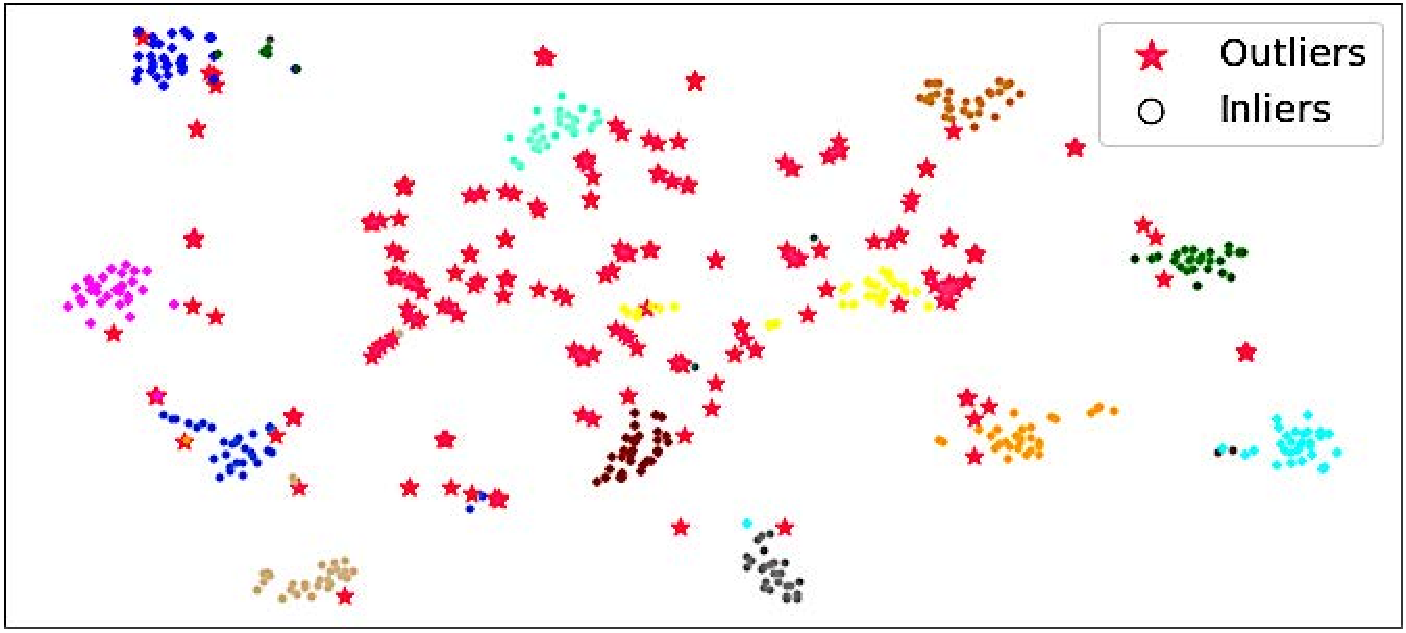
\includegraphics[width=.97\linewidth,height=0.152\textheight]{feat_base.pdf}
%   \caption{}
%   \label{fig:tsne_baseline}
\end{subfigure}
\begin{subfigure}{0.49\textwidth}
  \centering
  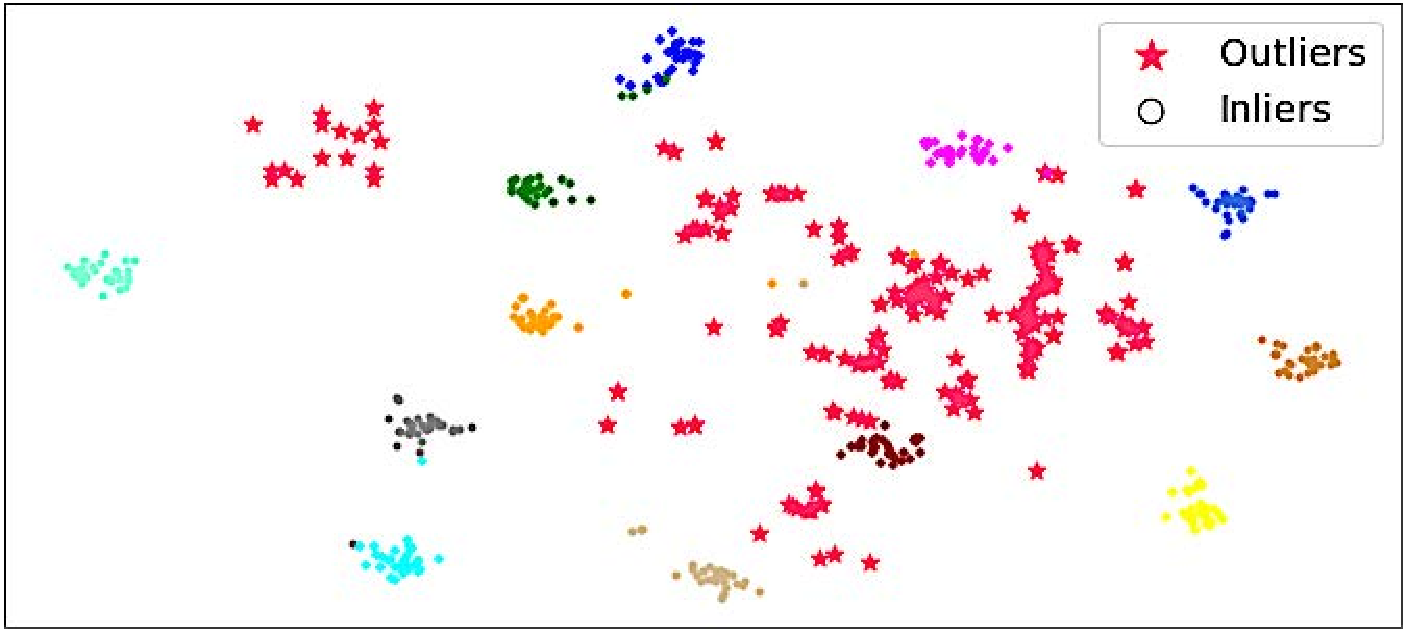
\includegraphics[width=.97\linewidth,height=0.152\textheight]{feat_visual.pdf}
%   \caption{}
%   \label{fig:tsne_ours}
\end{subfigure}
\vspace{-5pt}
\caption{t-SNE visualization of the learned embeddings of the test samples of CLINC150. Top: Previous $K$-way training; Bottom: Our proposed $(K+1)$-way training. Better view in color and enlarged.}
\label{fig:tsne}
\end{figure}
\end{abstract}


\section{Introduction}
%Conversational system is becoming an indispensable component in a variety of AI applications and acts as an interactive interface provided to users to improve user experience. Language understanding is crucial for conversational systems to provide appropriate responses to users. Intent classification is usually the first step of language understanding in these systems. Its primary goal is to identify diverse intentions behind user utterances and it is usually formalized as a classification problem. However, intent classes defined during training are inevitably inadequate to cover all of the user intents at the inference stage due to flexibility and randomness of the user utterances. Hence, out-of-scope (or unknown) intent classification is introduced to address this problem and it aims at building a classifier that can accurately identify supported (or known) intent classes while detecting out-of-scope (or unknown) intents that are unrelated to supported intents.


Conversational system is becoming an indispensable component in a variety of AI applications and acts as an interactive interface provided to users to improve user experience. Language understanding is essential for conversational systems to provide appropriate responses to users, and intent detection is usually the first step of language understanding. The primary goal is to identify diverse intentions behind user utterances, which is often formalized as a classification task. However, intent classes defined during training are inevitably inadequate to cover all possible user intents at the test stage due to the diversity and randomness of user utterances. Hence, out-of-scope (or unknown) intent detection is essential, which aims to develop a model that can accurately identify known (seen in training) intent classes while detecting the out-of-scope classes that are not encountered during training.

Due to the practical importance of out-of-scope intent detection, recent efforts have attempted to solve this problem by developing effective intent classification models. In general, previous works approach this problem by learning \emph{decision boundaries} for known intents and then using some confidence measure to distinguish known and unknown intents. For examples, LMCL~\citep{DBLP:conf/acl/LinX19} learns the decision boundaries with a margin-based optimization objective, and SEG~\citep{yan-etal-2020-unknown} assumes the known intent classes follow the distribution of mixture of Gaussians. After learning the decision boundaries, an off-the-shell outlier detection algorithm such as LOF~\citep{10.1145/335191.335388} is commonly employed to derive confidence scores  \cite{yan-etal-2020-unknown,DBLP:conf/emnlp/ShuXL17, DBLP:conf/acl/LinX19, DBLP:conf/iclr/HendrycksG17}.
If the confidence score of a test sample is lower than a predefined threshold, it is identified as an outlier. 

However, it may be problematic to learn decision boundaries solely based on the training examples of known intent classes. First, if there are sufficient training examples, the learned decision boundaries can be expected to generalize well on known intent classes, but not on the unknown. Therefore, extra steps are required in previous methods, such as using an additional outlier detection algorithm at the test stage or adjusting the confidence threshold by cross-validation. On the other hand, if there are not sufficient training examples, the learned boundaries may not generalize well on both known and unknown intents. As a result, these methods often underperform when not enough training data is given. Hence, it is important to provide learning signals of unknown intents at the training stage to overcome these limitations.

%is the key point of removing the constraints of previous methods. 

%In this paper, our goal is to remove these limitations and propose a simple yet effective method for out-of-scope intent detection.  We take a brave step to build pseudo out-of-scope examples directly to aid the training process. leading to the flexibility of selceting them.

In contrast to previous works, we adopt a different approach by explicitly modeling the distribution of unknown intents. Particularly, we construct a set of pseudo out-of-scope examples to aid the training process. We hypothesize that in the semantic feature space, real-world outliers can be well represented in two types: ``\emph{hard}'' outliers that are geometrically close to the inliers and ``\emph{easy}'' outliers that are distant from the inliners. For the ``hard'' ones, we construct them in a self-supervised manner by forming convex combination of the features of inliers from different classes. 
For the ``easy'' ones, the assumption is that they are very unrelated to the known intent classes, so they can be used to simulate the randomness and diversity of user utterances. They can be easily constructed using public datasets. For example, in our experiments, we randomly collect sentences from datasets of other NLP tasks such as question answering and sentiment analysis as open-domain outliers. 

In effect, by constructing pseudo outliers for the unknown class during training, we form a consistent $(K+1)$ classification task ($K$ known classes + 1 unknown class) for both training and test. Our model can be trained with a cross-entropy loss and directly applied to test data for intent classification and outlier detection without requiring any further steps.
As shown in Figure~\ref{fig:tsne} (better view in color and enlarged), our method can learn better utterance representations, which make each known intent class more compact and push the outliers away from the inliers. Our main contributions are summarized as follows.
\begin{itemize}
%\item We propose a novel model that is simple, efficient, and effective for out-of-scope intent detection by constructing pseudo outliers. We form a consistent (K+1) classification task for the training and test process to bridge the gap between fitting to training data and generalizing to test data.

\item We propose a novel out-of-scope intent detection approach by matching training and test tasks to bridge the gap between fitting to training data and generalizing to test data.

\item We propose to efficiently construct two types of pseudo outliers by using a simple self-supervised method and leveraging publicly available auxiliary datasets.

\item We conduct extensive experiments on four real-world dialogue datasets to demonstrate the effectiveness of our method and perform a detailed ablation study.
\end{itemize}


\section{Related Work}
\subsection{Out-of-Distribution Detection}
Early studies on outlier detection often adopt unsupervised clustering methods to detect malformed data~\citep{DBLP:journals/air/HodgeA04, chandola2009anomaly,zimek2012survey}. In recent years, a substantial body of work has been directed towards improving the generalization capacity of machine learning models on out-of-distribution (OOD) data~\citep{DBLP:journals/pieee/RuffKVMSKDM21, hendrycks2020many}. 
\citet{DBLP:conf/iclr/HendrycksG17} find that simple statistics derived from the outputting softmax probabilities of deep neural networks can be helpful for detecting OOD samples. Following this work, \citet{dcbe7abf4db64d1b89bf9802585660ed} propose to use temperature scaling and add small perturbation to input images to enlarge the gap between in-scope and OOD samples. 
\citet{lee2017training} propose to add a Kullback-Leibler divergence term in the loss function to encourage assigning lower maximum scores to OOD data. 
% \citet{lee2017training} used GAN~\citep{goodfellow2014generative} to detect out-of-scope images. Specifically, the discriminator in GAN is trained to produce low confidence scores for the out-of-scope samples.

Recently, there is a line of work that employs synthetic or real-world auxiliary datasets to provide learning signals for improving model robustness under various forms of distribution shift~\citep{DBLP:journals/corr/GoodfellowSS14,DBLP:journals/corr/abs-1907-07640,DBLP:conf/icml/HendrycksLM19,lee2017training}. Particularly, \citet{hendrycks2018deep} propose to leverage large-scale public datasets to represent outliers during training time and form a regularization term based on that. This idea is similar to our proposal of constructing open-domain outliers, but we use a simpler, end-to-end, $(K+1)$-way discriminative training procedure without any regularization term or threshold parameter.  

\begin{figure*}[t]
    \centering
    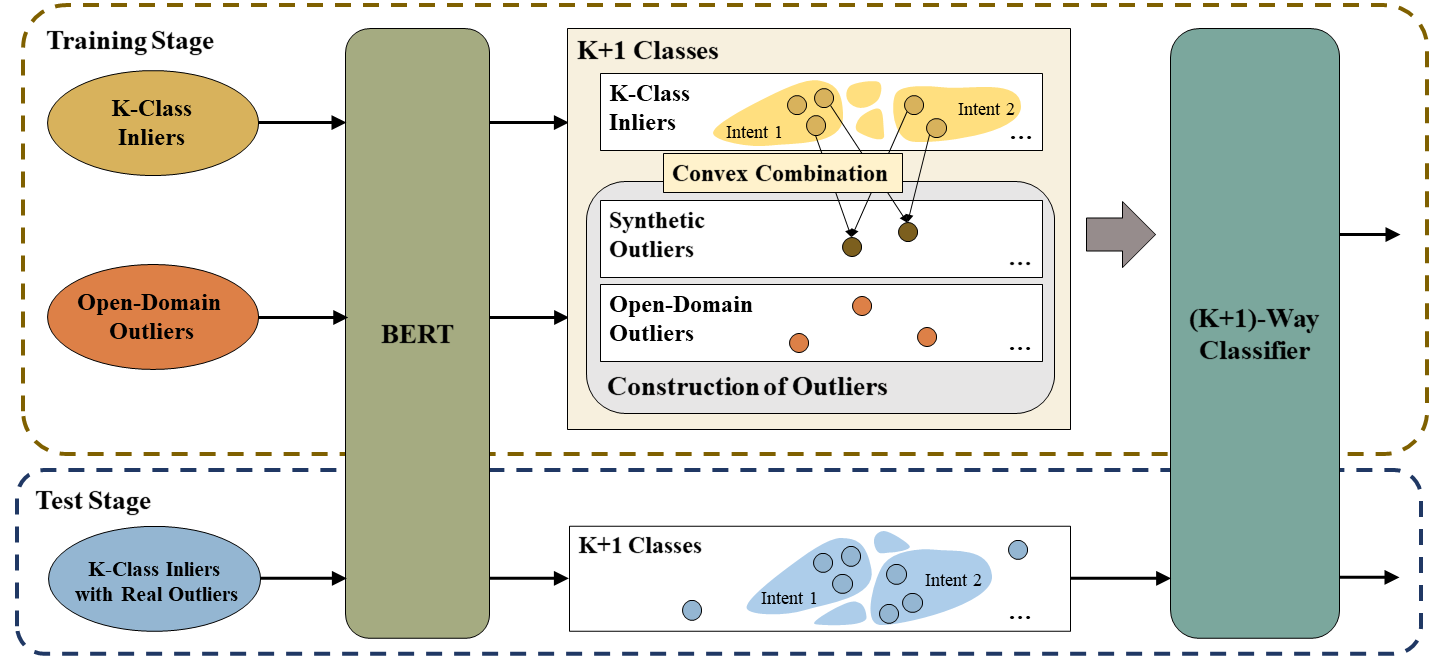
\includegraphics[width=150mm]{framework.png}
    \caption{An illustration of our proposed method. We use BERT as the utterance encoder. At training stage, we train a (K+1)-way classifier by constructing two types of pseudo outliers. The open-domain outliers are collected from an auxiliary dataset disjoint from both the training and test data. The synthetic self-supervised outliers are generated during training by random convex combinations of features of inliers from different known classes.}
    \label{fig:framework}
\end{figure*}
\subsection{Out-of-Scope Intent Detection}
While \citet{DBLP:conf/acl/HendrycksLWDKS20} find that pretrained transformer-based models like BERT are intrinsically more robust to OOD data, they suggest that there are still margins for improvement. Therefore, we build our model on top of BERT to improve intent detection under significant distribution shift. Previous methods for out-of-scope (or out-of-distribution) intent detection are commonly threshold-based, where models output a decision score and then compare it with a threshold that is predefined or selected by cross-validation. 

There are mainly three branches of related work. The first group uses a confidence score which determines the likelihood of an utterance being out-of-scope. 
For example, \citet{DBLP:conf/emnlp/ShuXL17} build $m$ binary Sigmoid classifiers for $m$ known classes respectively and select a threshold to reject OOD inputs that may have lower probabilities than the threshold across all $m$ classifiers. 
Similar to the OOD data generation method used in \citet{lee2017training}, \citet{ryu-etal-2018-domain} employ GAN~\citep{goodfellow2014generative} to generate simulated OOD examples with the generator and learn to reject simulated OOD examples with the discriminator.

The second group identifies out-of-scope sentences through reconstruction loss. For example, \citet{10.1016/j.patrec.2017.01.008} build an autoencoder to encode and decode in-scope utterances and obtain reconstruction loss by comparing input embeddings with decoded ones. Out-of-scope utterances result in higher reconstruction loss. 

The third group leverages off-the-shell outlier detection algorithms such as local outlier factor (LOF)~\citep{10.1145/335191.335388}, one-class SVM~\citep{6790022}, robust covariance estimators~\citep{article}, and isolation forest~\citep{10.1109/ICDM.2008.17} to detect out-of-scope examples. Utterance embeddings belonging to a specific class will be mapped to the corresponding cluster (usually modeled by a Gaussian distribution) while out-of-scope samples will be pushed away from all in-scope clusters. Examples of this kind include SEG~\citep{DBLP:conf/acl/YanFLLZWL20} and LMCL~\citep{DBLP:conf/acl/LinX19}. Very recently, \citet{Zhang_Xu_Lin_2021} propose to learn adaptive decision boundaries after pre-training instead of using off-the-shell outlier detection algorithms.
% in which they varied in methods to extract the sentence embedding.

In addition, some other work focuses on out-of-scope detection in few-shot scenarios. \citet{tan-etal-2019-domain} leverage independent source datasets as simulated OOD examples to form a hinge loss term. \citet{zhang-etal-2020-discriminative} propose to pretrain BERT by a natual language understanding task with large-scale training data to transfer useful information for few-shot intent detection. 

Finally, for our proposal of constructing synthetic outliers, the most similar method is {Mixup} proposed by \citet{DBLP:conf/iclr/ZhangCDL18}. However, their method is designed for data augmentation to enhance in-distribution performance and requires corresponding combinations in the label space \cite{DBLP:conf/nips/ThulasidasanCBB19}.

%which is essentially important as suggested by


% OOS in general:  
% Neural Network Based: MSP, Variational AutoEncoder, DOC, ODIN (CV).


% OOS in NLP: SEG, LMCL, VAGAN, Word Graph EMbedding, GAN-based, GDA + Mahalanobis distance, OOD for Low Resource. , AutoEncoder, Variational AutoEncoder



% Some defined Outlier Detection problem as binary classification problem. (AutoEncoder)
% Assumption: Open word / Close word Assumption


% Out-of-Domain Detection/Anomaly Detection/ Novelty Detection/ Out of Distribution Detection
%Category: (1) Reconstruction Loss; (2) Confidence Base (3) Outlier Detection / Distance Base
% Previous Studies:  GAN base (2) / Auto Encoder (1) / Variational Auto Encoder (1) / VAGAN (1) / LMCL (3) / SEG  (3) / ADB (3) / ODIN(2)/  MSP(2) / Word Graph Embedding (2) / DOC(
% Intent Classification: Associate utterance to intent, commonly by probability after Softmax
% Category (2) Set up a threshold and compare to the highest probability class. [MSP, ODIN(MSP with temperature scaling)]
% Category (1) Auto Encoder Base: Encode sentence embedding to a smaller hidden space and reconstruct it. Outlier sample produce higher reconstruction loss.  [Auto Encoder; Variational Auto Encoder; VAGAN]
% Category (3) Clustering Base; Treat OOS as outlier detection problem. [LMCL; SEG; ADB] 

%Intent classification has been broadly used by many dialog systems such as chat-bot with the task of predicting input utterance into one of the intents. Most of the studies focus on closed word assumption where no new intent will appears during testing. Traditional intent classification model classify utterance by using Soft-max activation function to acquire probability for each intent and output intent with highest probability. However, it is also critical to  detect out of  scope utterance as they will inevitably appears in dialog systems. With the capability to detect out of scope sentence, developers will be able to identify potential improvement and improve the flexibility of their dialog system.


\section{Methodology}


\paragraph{Problem Statement}
In a dialogue system, given $K$ predefined intent classes $S_{\text{known}}=\{C_i\}_{i=1}^K$, an unknown intent detection model aims at predicting the category of an utterance $u$, which may be one of the known intents or an out-of-scope intent $C_{\text{oos}}$. Essentially, it is a $K+1$ classification problem at the test stage. At the training stage, a set of $N$ labeled utterances $\mathcal{D}_{l} = \{ (x_i,c_i) \mid c_i\in S_{\text{known}})\}_{i=1}^{N}$ is provided for training. Previous methods typically train a $K$-way classifier for the known intents. %classes. 


% 之前的限制，idea怎么 ipsired的。overview怎么做的
\paragraph{Overview of Our Approach} 
%The discrepancy between training and inference results in additional complexity in previous methods. They usually require strong assumption on intent distribution (e.g., Gaussian mixture distribution) to build effective decision boundaries for each of known classes in the training stage. With the learned decision boundaries, in inference, outliers are usually detected by a post-step with the help of an additional off-the-shell outlier detector or hand-crafted confidence thresholding policy.  
The mismatch between the training and test tasks, i.e., $K$-way classification vs. $(K+1)$-way classification, leads to the use of strong assumptions and additional complexity in previous methods. Inspired by recent practice in meta learning to simulate test conditions in training~\citep{vinyals2016matching}, we propose to match the training and test settings. In essence, as shown in Figure~\ref{fig:framework}, we formalize a $(K+1)$-way classification task in the training stage by constructing out-of-scope samples via self-supervision and from open-domain data. Our method simply trains a $(K+1)$-way classifier without making any assumption on the data distribution. After training, the classifier can be readily applied to the test task without any adaptation or post-processing.
In the following, we elaborate on the details of our proposed method, including representation learning, construction of pseudo outliers, and discriminative training.
%In essence, we devise our method by ``a simple machine learning principle: test and train conditions must match''~\citep{vinyals2016matching}. 
%We intend to formalize a consistent $K+1$ classification task to bridge the gap between training and inference for our model.
%To this end, we propose an algorithm that only requires a single training stage with cross-entropy loss. 
% In result, we devise an effective unknown intent classification model that is simple and easy-to-train.

%As shown in Figure~\ref{fig:framework}, we build two kinds of outliers at training stage to form a consistent $K+1$ classification task for training and test, as described later. Note that following the conventional setting for unknown intent detection, we avoid utilizing any information from the outliers in the test set. After the training stage, our model can be readily applied to test examples without any further adaptation steps. In the following, we elaborate on how to construct outliers at the training stage and how to use them to aid the training process.




\subsection{Representation Learning}
We employ BERT~\citep{DBLP:conf/naacl/DevlinCLT19} -- a deep Transformer network as text encoder. Specifically, we take the $d$-dimensional output vector of the special classification token [CLS] as the representation of an utterance $u$, i.e.,
$$h = \text{BERT}(u) \in \mathbb{R}^d,$$ 
where $d=768$ by default. The training set $\mathcal{D}_{l}$ is then mapped to $\mathcal{D}_{l}^{tr} = \{(h_i, c_i)\mid h_i = \text{BERT}(u_i), (u_i, c_i)\in \mathcal{D}_{l}\}_{i=1}^N$ in the feature space.

%and an out-of-scope class $C_{oos}$ ,  where $c$ may either be in $S_{known}$ or an out-of-scope utterance, i.e., $c \in S = S_{known} \cup \{C_{OOS}\}$.  Note that as $S_{know n}$ varies, the coverage of $C_{oos}$ changes accordingly. 


%In a task-oriented dialog system, given $K$ predefined known intent classes $S_{known}=\{C_i\}_{i=1}^K$ and an out-of-scope class $C_{oos}$ , an unknown intent classification model aims at predicating the category $c$ of an utterance $u$, where $c$ may either be in $S_{known}$ or an out-of-scope utterance, i.e., $c \in S = S_{known} \cup \{C_{OOS}\}$.  Note that as $S_{know n}$ varies, the coverage of $C_{oos}$ changes accordingly. Given a labeled training set $\mathcal{D}_{l} = \{ (x_i,c_i) \mid c_i\in S_{known})\}_{i=1}^{N}$, previous methods consider a $K$-class classification problem in training whereas the targeted classes become $K+1$ during inference with an additional $C_{oos}$ class. 


%\subsection{The Proposed Method}



%为什么要两种类型。robust。simulate oos。模仿用户，再多一点 
\subsection{Construction of Outliers}\label{subsec: building outlier}

%We construct two different types of out-of-scope examples that are defined in terms of the complexity of recognizing them and generated dynamically in training. 

We construct two different types of pseudo outliers to be used in the training stage: synthetic outliers that are generated by self-supervision, and open-domain outliers that can be easily acquired. 

%At a high level, in the learned representation space, we hypothesize that the outliers that are similar to inliers drawn from known intent classes may be geometrically \emph{close} to these inliers. We call this kind of outliers as the \emph{hard} ones.  

%On other hand, in practical, despite dialog systems are task-oriented, but users are not. Generally, users can input anything they want into the system such as unrelated small talks, typos, or punctuation. We regard this kind of outliers as the \emph{easy} ones.

%To enhance the generalization ability of our model, we devise the corresponding construction methods for these two kinds of outliers.  

\paragraph{Synthetic Outliers by Self-Supervision} To improve the generalization ability of the unknown intent detection model, we propose to generate ``\emph{hard}'' outliers in the feature space, which may have similar representations to the inliers of known intent classes. We hypothesize that those outliers may be geometrically \emph{close} to the inliers in the feature space. Based on this assumption, we propose a self-supervised method to generate the ``hard'' outliers using the training set $\mathcal{D}^{tr}_{l}$.  

%We call this kind of outliers as the \emph{hard} ones.
%Based on our geometrically \emph{close} hypothesis in the representation space, the \emph{hard} outliers can be generated based on information provided by the training set $\mathcal{D}^{tr}_{l}$. 
%We consider generating this kind of hard outliers that resemble the known intent examples in a self-supervised manner. 
Specifically, in the feature space, we generate synthetic outliers by using convex combinations of the features of  inliers from different intent classes:
\begin{flalign}
\begin{aligned}
	h^{oos} =\theta * h_{\beta} + (1-\theta)*h_{\alpha},
\end{aligned}
\end{flalign}
where $h_{\beta}$ and $h_{\alpha}$ are the representations of two utterances which are randomly sampled from different intent classes in $\mathcal{D}_{l}^{tr}$, i.e., $c_{\beta} \neq c_{\alpha}$, and $h^{oos}$ is the synthetic outlier. For example, $\theta$ can be sampled from a uniform distribution $U(0, 1)$. In this case, when $\theta$ is close to $0$ or $1$, it will generate ``harder'' outliers that only contain a small proportion of mix-up from different classes. In essence, ``hard'' outliers act like support vectors in SVM~\citep{cortes1995support}, and ``harder'' outliers could help to train a more discriminative classifier. 

%We find that $\theta$ that is close to $0$ or $1$ is important, which indicates that a small proportion of mixup from different classes can lead to distinctive features.
% To ensure $h^{oos}$ is a possible outlier, the weight parameter $\theta$ should not be too close to 0 or 1.
%namely $\mathbf{\theta} \sim \mathcal{U}(0.2, 0.8)$. 

The generated outliers $h^{oos}$ are assigned to the class of $C_{oos}$, the $(K+1)$-th class in the feature space, forming a training set
\begin{flalign}
\begin{aligned}
	\mathcal{D}_{co}^{tr} = \{(h_{i}^{oos}, c_i = C_{oos}) \}_{i=1}^{M}.
\end{aligned}
\end{flalign}
Notice that since the outliers are generated in the feature space, it is very efficient to construct a large outlier set $\mathcal{D}_{co}^{tr}$.

%than $\mathcal{D}_{l}^{tr}$.

%By assigning all of the generated $h^{oos}$ into the class of $C_{oos}$, we get an out-of-scope set for training in the embedded space: 
 

\paragraph{Open-Domain Outliers} In practical dialogue systems, user input can be arbitrary free-form sentences. To simulate real-world outliers and provide learning signals representing them in training, we propose to construct a set of open-domain outliers, which can be easily obtained. Specifically, the set of free-form outliers $\mathcal{D}_{fo}$ can be constructed by collecting sentences from various public datasets that are disjoint from the training and test tasks. There are many datasets available, including the question answering dataset SQuaD 2.0~\citep{DBLP:conf/acl/RajpurkarJL18}, the sentiment analysis datasets Yelp~\citep{DBLP:conf/cikm/MengSZ018} and IMDB~\citep{DBLP:conf/acl/MaasDPHNP11}, and dialogue datasets from different domains. 

In the feature space, $\mathcal{D}_{fo}$ is mapped to
$\mathcal{D}_{fo}^{tr} = \{(h^{oos}_i, c_i=C_{oos})\mid h^{oos}_i=\text{BERT}(u_i), u_i \in \mathcal{D}_{fo}\}_{i=1}^H$.

Both synthetic outliers and open-domain outliers are easy to construct. As will be demonstrated in Section~\ref{sec:exp}, both of them are useful, but synthetic outliers are much more effective than open-domain outliers in improving the generalization ability of the trained $(K+1)$-way intent classifier. 

%To simulate real-world outliers, we propose to construct another set of open-domain outliers. In practice, despite dialog systems are task-oriented, but users are not. Generally, users can input anything they want into the system such as unrelated small talks, typos, or punctuation. We regard this kind of outliers as the \emph{easy} ones.
%Next, we consider another set of easy-to-recognized out-of-scope utterances. We construct an easy-acquired OOS set so as to provide learning signals representing this kind of free-form utterances. Specifically, we build an OOS set $\mathcal{D}_{fo}$ which consists of $0.5$ million utterances by collecting sentences from the question answering dataset SQuaD 2.0~\citep{DBLP:conf/acl/RajpurkarJL18} and the sentiment analysis datasets Yelp~\citep{DBLP:conf/cikm/MengSZ018} and IMDB~\citep{DBLP:conf/acl/MaasDPHNP11}. The corresponding set is noted as
%$\mathcal{D}_{fo}^{tr} = \{(h^{oos}_i, c_i=C_{oos})\mid h^{oos}_i=\text{BERT}(u_i), u_i \in \mathcal{D}_{fo}\}_{i=1}^H$.


\subsection{Discriminative Training}

After constructing the pseudo outliers, in the feature space, our training set $\mathcal{D}^{tr}$ now consists of a set of inliers $\mathcal{D}_{l}^{tr}$ and two sets of outliers $\mathcal{D}_{co}^{tr}$ and $\mathcal{D}_{fo}^{tr}$, i.e., $\mathcal{D}^{tr} = \mathcal{D}_{l}^{tr} \cup \mathcal{D}_{co}^{tr} \cup \mathcal{D}_{fo}^{tr}$ and $|\mathcal{D}^{tr}| = N+M+H$. Therefore, in the training stage, we can train a $(K+1)$-way classifier  with the intent label set $S= S_{known} \cup \{C_{oos}\}$, which can be directly applied in the test stage to identify unknown intent and classify known ones. In particular, we use a multilayer perceptron network, $\Phi(\cdot)$, as the classifier in the feature space. The selection of the classifier is flexible, and the only requirement is that it is differentiable. Then, we train our model using a cross-entropy loss:
\begin{align*}
	\mathcal{L} = 
	- \frac{1}{|\mathcal{D}^{tr}|}\sum_{\mathcal{D}^{tr}}\log \frac{\exp(\Phi(h_i)^{c_i}/\tau)}{\sum_{j\in S}\exp(\Phi(h_i)^j/\tau)},
\end{align*}
where $\Phi(h_i)^{c_i}$ refers to the output logit of $\Phi(\cdot)$ for the ground-truth class $c_i$, and $\tau \in \mathbb{R}^+$ is an adjustable scalar temperature parameter.





\section{Experiments}\label{sec:exp}
%更换squad。
\begin{table*}[ht!]
\centering
\scalebox{0.85}{
\begin{tabular}{cc|cc|cc|cc|cc}
\specialrule{0.1em}{0.2em}{0.2em}
\multicolumn{2}{c}{}&\multicolumn{2}{c}{CLINC150}&\multicolumn{2}{c}{StackOverflow}&\multicolumn{2}{c}{Banking}&\multicolumn{2}{c}{M-CID-EN}\\
&Methods & Accuracy & Macro-F1& Accuracy & Macro-F1& Accuracy & Macro-F1& Accuracy & Macro-F1\\
\specialrule{0.05em}{0.1em}{0.2em}
\multirow{6}{*}{25\%} 
                    &MSP&66.60 & 51.20 &33.94 &45.68  &48.15 &48.47 &52.05&43.14   \\
                    &DOC&64.43 & 44.60 &60.68 &60.51  &37.78 &46.35 &49.32&46.59  \\
                    &SEG&72.86 & 65.44 &47.00 &52.83  &51.11 &55.68 &44.51&50.14 \\
                    &LMCL& 68.57&62.42 &41.60 &48.21  &52.77 &56.73 &41.44&46.99  \\
                    &Softmax&76.50& 67.74 &46.17 &50.78  &57.88 & 58.32&41.95&45.46   \\
                    % &\bf {Ours} &\bf88.39 & \bf 74.49 &\bf79.88 & \bf 69.46 & \bf 82.15&\bf 67.96&\bf 78.38&\bf 69.83\\
                    &\bf {Ours} &\bf88.44 & \bf 80.73 &\bf68.74 & \bf 65.64 & \bf 74.11&\bf 69.93&\bf 87.08&\bf 79.67\\
\specialrule{0.05em}{0.1em}{0.2em}
\multirow{6}{*}{50\%} 
                    &MSP& 68.61& 51.20 &56.33 &62.92  &53.83 &65.33 &61.21&54.33  \\
                    &DOC& 62.46 & 70.01  &61.62 &68.97  &58.29 &57.30  &59.97&62.28 \\
                    &SEG& 77.05 & 79.42 & 68.50 & 74.18 &68.44 &76.48  &67.91&72.37 \\
                    &LMCL& 78.63& 80.42 &64.34 &71.80 & 63.59 &73.99 &63.42&69.04  \\
                    &Softmax&82.47&82.86 &65.96 &71.94  &67.44 &74.19 &64.72&69.35 \\
                    % &\bf {Ours}&\bf 85.44 &\bf 84.17 &\bf 78.17 &\bf 79.16 & \bf 74.91&\bf 77.34&\bf74.19&\bf75.12\\
                    &\bf {Ours}&\bf 88.33 &\bf 86.67 &\bf 75.08 &\bf 78.55 & \bf 72.69&\bf 79.21&\bf81.05&\bf79.73\\
\specialrule{0.05em}{0.1em}{0.2em}
\multirow{6}{*}{75\%} 
                    &MSP&73.41 &81.81  &76.73 & 77.63 &71.92 &80.77 &72.89&77.34  \\
                    &DOC&74.63 & 78.63 & 63.98 &62.07  &72.02 &78.04 &69.79&71.18  \\
                    &SEG&81.92 & 86.57  &80.83 &84.78  &78.87 &85.66 &75.73&79.97 \\
                    &LMCL& 84.59&88.21 &80.02 & 84.47  &78.66 &85.33 &77.11&80.96  \\
                    &Softmax& 86.26& 89.01 &77.41 &82.28  &78.20 &84.31 &76.99& 80.82 \\
                    % &\bf {Ours}&\bf85.08 & 86.30 &\bf81.08 & \bf85.11 &\bf79.32 &84.66&\bf77.14&79.53\\
                    &\bf {Ours}&\bf88.08 & \bf89.43 &\bf81.71 & \bf85.85 &\bf81.07 &\bf86.98&\bf80.24&\bf82.75\\
\specialrule{0.1em}{0.1em}{0.2em}
\end{tabular}
}
\caption{\label{mainresult1}
Overall accuracy and macro f1-score for unknown intent detection with different proportion of seen classes. For each setting, the best result is marked in bold. 
% For the 75\% setting, the top 2 results for each metric are marked in bold.
}
\end{table*}
In this section, we present the experimental results of our proposed method on the targeted task of unknown intent detection. Given a test set comprised of known and unknown intent classes, the primary goal of an unknown intent detection model is to assign correct intent labels to utterances in the test set. Notice that the unknown intent label $C_{oos}$ is also included as a special class for prediction. 
\begin{table}
\centering
% \setlength{\tabcolsep}{1.5pt}
% \footnotesize
\scalebox{0.76}{
\begin{tabular}{l|c|c|c|c}
\specialrule{0.05em}{0.1em}{0.2em}
Dataset & Vocab & Avg. Length & Samples & Classes\\
\specialrule{0.05em}{0.1em}{0.2em}
CLINC150&8,376&8.31&23,700&150\\
StackOverflow&17,182&9.18&20,000&20\\
Banking&5028&11.9&13,083&77\\
M-CID-EN&1,254&6.74&1,745&16\\
\specialrule{0.05em}{0.1em}{0.2em}
\end{tabular}
}
\caption{\label{table:datsets_stats}
Dataset statistics.
}
\end{table}

\begin{table*}[t]
\centering
\scalebox{0.90}{
\begin{tabular}{cc|cc|cc|cc|cc}
\specialrule{0.1em}{0.2em}{0.2em}
\multicolumn{2}{c}{}&\multicolumn{2}{c}{CLINC150}&\multicolumn{2}{c}{StackOverflow}&\multicolumn{2}{c}{Banking}&\multicolumn{2}{c}{M-CID-EN}\\
&Methods & Unknown & Known& Unknown & Known& Unknown & Known& Unknown & Known\\
\specialrule{0.05em}{0.1em}{0.2em}
\multirow{6}{*}{25\%} 
                    &MSP&73.20 &50.62  &22.59 &50.30  &49.98 &48.39 &56.27&37.86  \\
                    &DOC&71.08 &43.91  &66.11 &59.39  &31.41 &47.14  &53.08&44.92 \\
                    &SEG&79.90 &65.06  &46.17 &54.16  &53.22 &55.81 &42.73&51.99  \\
                    &LMCL&75.61 &62.01  &38.85 &50.15 &55.29 &56.81  &36.99&49.50 \\
                    &Softmax&83.04 &67.34  &45.52 &51.83  &62.52 &58.10 &35.39&46.22  \\
                    % &\bf {Ours} &\bf92.64 & \bf74.02 &\bf85.79 & \bf66.20 & \bf87.87&\bf67.00&\bf84.37&\bf66.20\\
                    &\bf {Ours} &\bf92.35 & \bf80.43 &\bf74.86 & \bf63.80 & \bf80.12&\bf69.39&\bf91.15&\bf76.80\\
\specialrule{0.05em}{0.1em}{0.2em}
\multirow{6}{*}{50\%} 
                    &MSP&57.78 &68.03  &35.18 &70.09  &29.31 &66.28 &58.55&53.80  \\
                    &DOC&57.62 &70.17  &47.96 &71.07  &49.88 &57.50  &47.22&64.16 \\
                    &SEG&78.02 &79.43  &60.89 &75.51 &60.42 &76.90&61.04 &73.80\\
                    &LMCL&79.89 &80.42  &53.12 &71.80  &50.30 &74.62  &51.11&71.29 \\
                    &Softmax&84.19 &82.84  &56.80 &73.45  &60.28 &74.56 &56.30&70.98  \\
                    % &\bf {Ours}&\bf87.48 &\bf84.12 &\bf77.68 &\bf79.31 & \bf73.91&\bf77.43&\bf73.50&\bf75.32\\
                    &\bf {Ours}&\bf90.30 &\bf86.54 &\bf71.88 &\bf79.22 & \bf67.26&\bf79.52&\bf82.44&\bf79.39\\
\specialrule{0.05em}{0.1em}{0.2em}
\multirow{6}{*}{75\%} 
                    &MSP&57.83 &82.02  &41.73 &80.03  &23.86 &81.75 &39.56&80.50  \\
                    &DOC&64.62 &78.76  &49.50&62.91  &39.47 &78.72 &49.41&72.99  \\
                    &SEG&76.12 &86.67  &62.30 &86.28  &54.43 &86.20 &51.51&82.34  \\
                    &LMCL&80.42 &88.28  &61.40 &84.47  &53.26 &85.89  &54.61&83.16 \\
                    &Softmax&83.12 &\bf89.61  &54.07&84.11  &56.90 &84.78 &58.73&82.66  \\
                    % &\bf {Ours}&\bf82.35 & 86.33 &\bf65.51 & \bf86.36 &\bf63.42 &85.03&\bf62.50&80.95\\
                    &\bf {Ours}&\bf86.28 &89.46 &\bf65.44 & \bf87.22 &\bf60.71 &\bf87.47&\bf69.00&\bf83.89\\
\specialrule{0.1em}{0.1em}{0.2em}
\end{tabular}
}
\caption{\label{mainresult2}
Macro f1-score of the known classes and f1-score of the unknown class with different proportion of seen classes. For each setting, the best result is marked in bold.
%For the 25\% and 50\% settings, the top 1 results for each metric are marked in bold. For the 75\% setting, the top 2 results for each metric are marked in bold.
}
\end{table*}
\subsection{Datasets and Baselines}
% \begin{figure*}[t]
%     \centering
%     \includegraphics[width=130mm]{number_ablation.png}
%     \caption{A study of the numbers of generated outliers.}
%     \label{fig:number_ablation}
% \end{figure*}

% We evaluate our proposed method on $4$ real task-oriented dialogueue datasets: CLINC150~\citep{larson2019evaluation}, StackOverflow~\citep{DBLP:conf/naacl/XuWTXZWH15}, Banking~\citep{DBLP:journals/corr/abs-2003-04807}, and M-CID-EN~\citep{arora2020cross}. The detailed statistics of datasets are summarized in Table~\ref{table:datsets_stats}. 
We evaluate our proposed method on four benchmark datasets as follows, three of which are newly released dialogue datasets designed for intent detection. The statistics of the datasets are summarized in Table~\ref{table:datsets_stats}. 

\textbf{CLINC150}~\citep{larson2019evaluation} is a dataset specially designed for out-of-scope intent detection, which consists of $150$ known intent classes from $10$ domains. The dataset includes $22,500$ in-scope queries and $1,200$ out-of-scope queries. For the in-scope ones, we follow the original splitting, i.e., $15,000$, $3,000$ and $4,500$ for training, validation, and testing respectively. For the out-of-scope ones, we group all of the $1,200$ queries into the test set. 

\textbf{StackOverflow}~\citep{DBLP:conf/naacl/XuWTXZWH15} consists of $20$ classes with $1,000$ examples in each class. We follow the original splitting, i.e., $12,000$ for training, $2,000$ for validation, and $6,000$ for test.

\textbf{Banking}~\citep{DBLP:journals/corr/abs-2003-04807} is a fine-grained intent detection dataset in the banking domain. It consists of $9,003$, $1,000$, and $3,080$ user queries in the training, validation, and test sets respectively.

% \textbf{M-CID}~\citep{arora2020cross} is a recently released multilingual intent detection dataset related to Covid-$19$, which consists of $1,745$ English utterances covering $16$ intent classes. We note the English subset of this dataset as M-CID-EN and use it in our experiments. The splitting of M-CID-EN is $1,258$ for training, $148$ for validation, and $339$ for test. 
\textbf{M-CID}~\citep{arora2020cross} is a recently released dataset related to Covid-$19$. We use the English subset of this dataset referred to as M-CID-EN in our experiments, which covers $16$ intent classes. The splitting of M-CID-EN is $1,258$ for training, $148$ for validation, and $339$ for test. 

We extensively compare our method with the following unknown intent detection methods.
\begin{itemize}
\item \textbf{Maximum Softmax Probability (MSP)}~\citep{DBLP:conf/iclr/HendrycksG17} employs the confidence score derived from the maximum softmax probability to predict the class of a sample. The idea under the hood is that the lower the confidence score is, the more likely the sample is of an unknown intent class.

\item \textbf{DOC}~\citep{DBLP:conf/emnlp/ShuXL17} considers to construct $m$ $1$-vs-rest sigmoid classifiers for $m$ seen classes respectively. It uses the maximum probability from these classifiers as the confidence score to conduct classification.

\item \textbf{SEG}~\citep{DBLP:conf/acl/YanFLLZWL20} models the intent distribution as a margin-constrained Gaussian mixture distribution and uses an additional outlier detector -- local outlier factor (LOF)~\citep{10.1145/335191.335388} to achieve unknown intent detection. 

\item \textbf{LMCL}~\citep{DBLP:conf/acl/LinX19} considers to learn discriminative embeddings with a large margin cosine loss. It also uses LOF as the outlier detection algorithm.

\item \textbf{Softmax}~\citep{DBLP:conf/acl/YanFLLZWL20} uses a softmax loss to learn discriminative features based on the training dataset, which also requires an additional outlier detector such as LOF for detecting the unknown intents. 
\end{itemize}

\begin{figure*}[t]
\begin{subfigure}{0.32\textwidth}
  \centering
  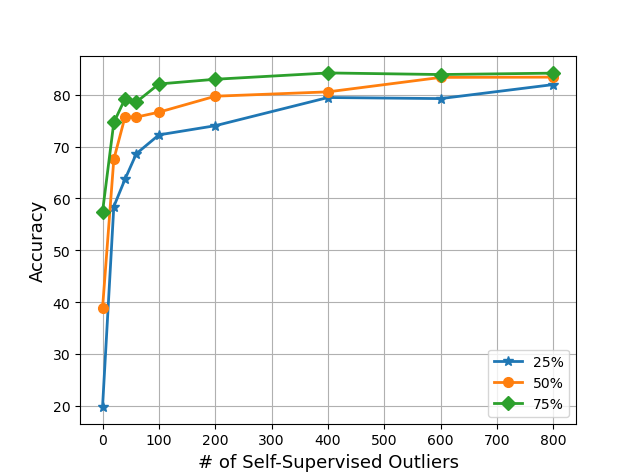
\includegraphics[width=1.1\linewidth]{acc_convex_new.png}
  \caption{ }
  \label{fig:convex_acc}
\end{subfigure}%
\begin{subfigure}{0.32\textwidth}
  \centering
  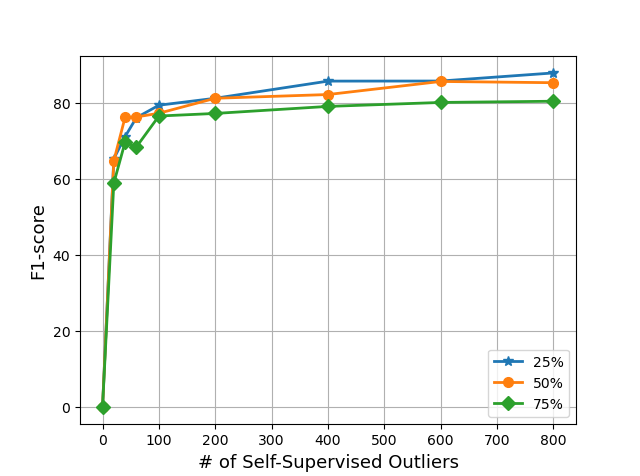
\includegraphics[width=1.1\linewidth]{F1_oos_convex_new.png}
  \caption{}
  \label{fig:convex_f1_unknown}
\end{subfigure}%
\begin{subfigure}{.32\textwidth}
  \centering
  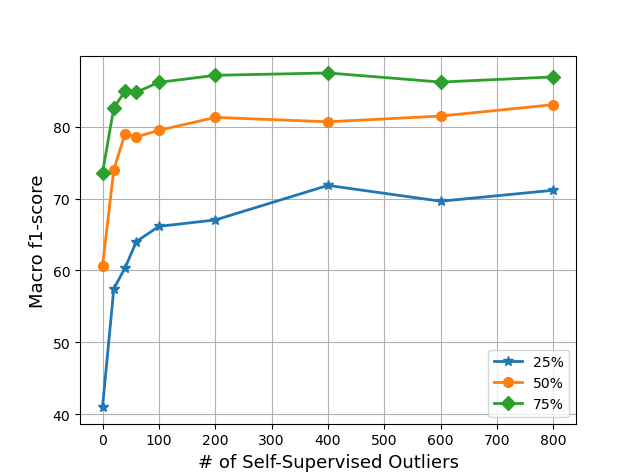
\includegraphics[width=1.1\linewidth]{macro_f1_convex_new.png}
  \caption{}
  \label{fig:convex_f1}
\end{subfigure}

\begin{subfigure}{.32\textwidth}
  \centering
  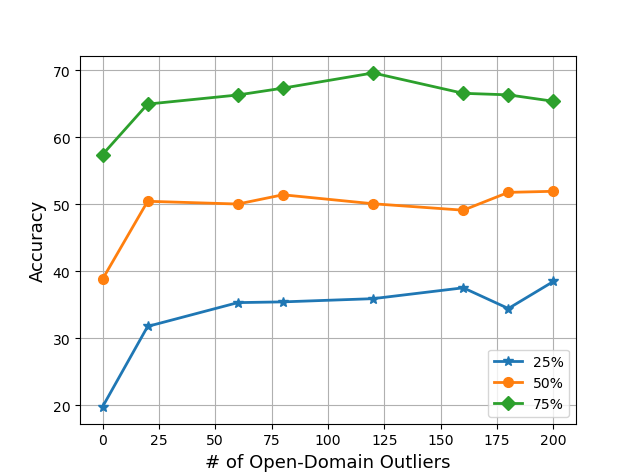
\includegraphics[width=1.1\linewidth]{acc_open_new.png}
  \caption{}
  \label{fig:open_domain_acc}
\end{subfigure}%
\begin{subfigure}{.32\textwidth}
  \centering
  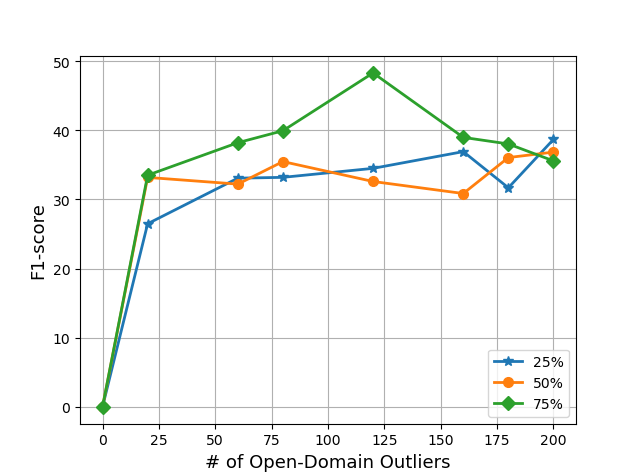
\includegraphics[width=1.1\linewidth]{f1_oos_open_new.png}
  \caption{}
  \label{fig:open_domain_f1_unknown}
\end{subfigure}%
\begin{subfigure}{.32\textwidth}
  \centering
  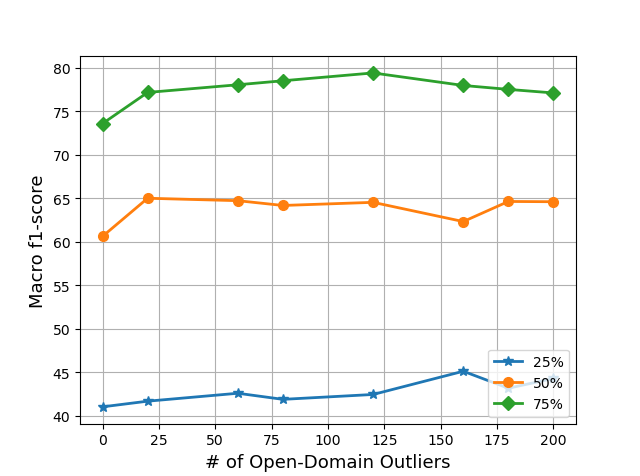
\includegraphics[width=1.1\linewidth]{macro_f1_open_new.png}
  \caption{}
  \label{fig:open_domain_f1}
\end{subfigure}
\caption{Effect of the number of pseudo outliers on CLINC150. %Sub-figures \ref{fig:convex_acc}, \ref{fig:convex_f1_unknown} and \ref{fig:convex_f1} 
(a), (b), and (c) display overall accuracy, f1-score on the unknown class and overall macro f1-score with varying number of self-supervised outliers respectively. 
%Sub-figures \ref{fig:open_domain_acc}, \ref{fig:open_domain_f1_unknown} and \ref{fig:open_domain_f1} 
(d), (e), and (f) display the corresponding results with varying number of open-domain outliers.}
% ,,
\label{fig:numbers}
\end{figure*}
\subsection{Experimental Setup and Evaluation Metrics}
To compare with existing methods, we follow the setting in LMCL~\citep{DBLP:conf/acl/LinX19}. Specifically, for each dataset, we randomly sample $75\%$, $50\%$, and $25\%$ of the intent classes from the training set as the known classes to conduct training, and we set aside the rest as the unknown classes for test. 
% Notice that for training and validation, we only use examples within the chosen known classes and our generated pseudo outliers.
Notice that for training and validation, we only use data within the chosen known classes and do not expose our model to any of test-time outliers. 
% Unless otherwise specified, in each training batch, we generate $\sim150$ and $800$ examples for the open-domain and self-supervised outliers respectively.
Unless otherwise specified, in each training batch, we keep the ratio of inliers, open-domain outliers and self-supervised outliers roughly as $1:1:4$. This setting is empirically chosen and affected by the memory limit of NVIDIA 2080TI GPU, which we use for conducting the experiments. The number of pseudo outliers can be adjusted according to different environments, and a larger number of self-supervised outliers typically takes more time to converge.
% and the number of labeled examples is selected according to the capacity of GPUs.

We use Pytorch~\citep{DBLP:conf/nips/PaszkeGMLBCKLGA19} as the backend to conduct the experiments. We use the pretrained BERT mdoel (\emph{bert-base-uncased}) provided by~\citet{wolf2019huggingface} as the encoder for utterances. We use the output vector of the special classification token [CLS] as the utterance embedding and fix its dimension as $768$ by default throughout all of our experiments. To ensure a fair comparison, all baselines and our model use the same encoder. 

%For the utterance representation of our model and baselines, our encoder is the pretrained BERT mdoel of \emph{bert-base-uncased} provided by~\citep{wolf2019huggingface}.

% In addition, we set the max length of input sentences for BERT as $30$, $45$, $55$, and $25$ for CLINC150, StackOverflow, Banking, and M-CID-EN respectively. 

For model optimization, we use AdamW provided by \citet{wolf2019huggingface} to fine-tune BERT and Adam proposed by \citet{DBLP:journals/corr/KingmaB14} to train the MLP clasisfier $\Phi(\cdot)$. We set the learning rate for BERT as $1e^{-5}$ as suggested by \citet{DBLP:conf/naacl/DevlinCLT19}. For the MLP clasisfier, the learning rate is fixed as $1e^{-4}$. Notice that the fine-tuning of BERT is conducted simultaneously with the training of the classifier $\Phi(\cdot)$ with the same cross-entropy loss. 
The MLP classifier $\Phi(\cdot)$ has a two-layer architecture with [$1024$, $1024$] as hidden units.
The temperature parameter $\tau$ is selected by cross-validation and set as $0.1$ in all experiments.

Following LMCL~\citep{DBLP:conf/acl/LinX19}, we use overall accuracy and macro f1-score as evaluation metrics. All results reported in this section are the average of $10$ runs with different random seeds, and each run is stopped until reaching a plateau on the validation set. For baselines, we follow their original training settings except using the aforementioned BERT as text encoder.  
\begin{figure}
  \centering
  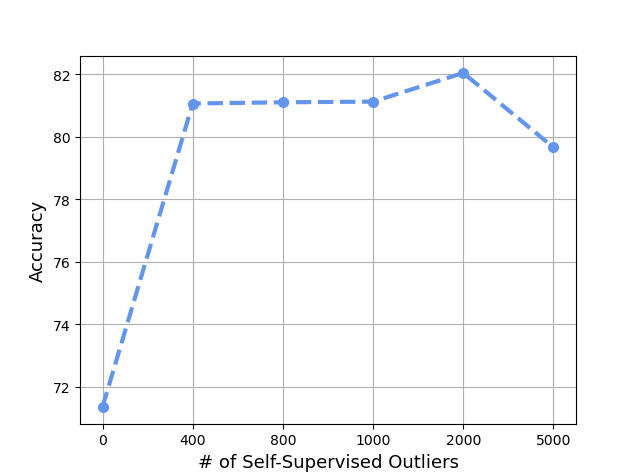
\includegraphics[width=1.\linewidth,height=0.19\textheight]{num_convex.png}
%\caption{Accuracy of the 75\% setting of Banking with different number of self-supervised outliers and the number of open-domain outliers fixed to $100$.}
\caption{Effect of the number of self-supervised outliers on overall intent detection accuracy under the 75\% setting of Banking.}
\label{fig:convex_num}
\end{figure}

\subsection{Result Analysis}
We present our main results in Table~\ref{mainresult1} and Table~\ref{mainresult2}. Specifically, Table~\ref{mainresult1} gives results in overall accuracy and macro f1-score for all classes including the outlier class, while Table~\ref{mainresult2} shows results in macro f1-score for the known classes and f1-score for the outlier class respectively. It can be seen that, on all benchmarks and in almost every setting, our model significantly outperforms the baselines. As shown in Table~\ref{mainresult2}, our method achieves favorable performance on both unknown and known intent classes simultaneously.

It is worth mentioning that the large improvements of our method in scenarios with small labeled training sets (25\% and 50\% settings) indicate its great potential in real-life applications, since a practical dialogue system often needs to deal with a larger proportion of outliers than inliers due to different user demographic, ignorance/unfamiliarity of/with the platform, and limited intent classes recognized by the system (especially at the early development stage). 
% As shown in Table~\ref{mainresult2}, our method can achieve favorable performance on both unknown and known intents simultaneously.
% because annotated training sets can be expensive and laborious to collect for dialogue systems and our goal is to recognize a finite group of known objects in myriad unknown objects~\citep{DBLP:journals/pami/ScheirerRSB13}.
%It is often the case that in real-life dialogue systems, training sets with labeled intents can be laborious to collect.The significant superiority of our method in scenarios with small labeled training sets demonstrates the great potential of our proposed method to be applied in real-life productions. Our method can achieve favorable performance not only for unknown intents but also for known intents.
% On the other hand, as shown in Table~\ref{mainresult1}, we can see that in the $75\%$ setting, our method is still among the best in accuracy, but slightly outperformed by some baselines in f1-score in several cases. However, as shown in Table~\ref{mainresult2}, when comparing with SEG, LMCL, and Softmax, it can be seen that their advantages are mainly in the known classes. However, our method can outperform them on the unknown classes. Take SEG and LMCL for example, they are all margin-based methods with different assumptions on intent distribution. As the proportion of known intents increases, they can better model known intents, which indicates they are more data-dependent. In contrast, we can achieve comparable results without relying on additional outlier detector, tuning margin, and conducting threshold selection.

More importantly, referring to Table~\ref{mainresult2}, as the proportion of known intents increases, it can be seen that the performance gains of the baselines mainly lie in the known classes. In contrast, our method can strike a better balance between the known and unknown classes without relying on additional outlier detector, margin tuning, and threshold selection, demonstrating its high effectiveness and generality. 
Take the Softmax baseline for example, in the $75\%$ case of CLINC150, it achieves a slightly higher result than our model on the known classes but a substantially lower result on the unknown ones. 
% Take SEG and LMCL for example, they are all margin-based methods with different assumptions on intent distribution. 
% As the proportion of known intents increases, they can better model known intents, which indicates they are more data-dependent. 
% In contrast, we can achieve comparable results without relying on additional outlier detector, tuning margin, and conducting threshold selection.

\subsection{Effect of Pseudo Outliers}
We conduct an ablation study on the effectiveness of the two kinds of pseudo outliers and summarize the results in Table~\ref{table:ablation}. The first row of the three settings ($25\%$, $50\%$, and $75\%$) stands for training solely with the labeled examples of CLINC150 without using any pseudo outliers. In general, self-supervised synthetic outliers and open-domain outliers both lead to positive effects on classification performance. For each setting, comparing the second row with the third, we can observe that the synthetic outliers produced by convex combinations lead to a much larger performance gain than that of pre-collected open-domain outliers. Finally, combining them for training leads to the best results, as shown in the fourth row of each setting.

Next, we conduct experiments to study the impact of varying the number of the two kinds of pseudo outliers separately, as shown in Figure~\ref{fig:numbers}. We first fix the number of open-domain outliers as zero and then increase the number of self-supervised outliers. The results are displayed in Figure~\ref{fig:numbers} (a), (b) and (c). In particular, as the number of self-supervised outliers grows, the performance first increases quickly and then grows slowly. On the other hand, we fix the number of self-supervised outliers as zero and then increases the number of open-domain outliers. The results are shown in Figure~\ref{fig:numbers}  (d), (e) and (f), where it can be seen that dozens of open-domain outliers already can bring significant improvements, though the gain is much smaller compared to that of the self-supervised outliers.

Finally, we investigate the impact of the number of self-supervised outliers on overall intent detection accuracy with both the number of inliers and the number of open-domain outliers fixed as 100 per training batch. %Results for accuracy of the $75\%$ Banking scenario are presented 
As shown in Figure~\ref{fig:convex_num}, we increase the number of self-supervised outliers from 0 to $5000$. Note that $400$ is the default setting used in Table~\ref{mainresult1} and Table~\ref{mainresult2}. We can see that comparable results can be obtained for a wide range of numbers. However, when the number grows to $5000$, the performance exhibits a significant drop. We hypothesize that as the number increases, the generated synthetic outliers may be less accurate, because some convex combinations may fall within the scope of known classes.

%the sampling density gets denser and 

To summarize, self-supervised outliers play a much more important role than open-domain outliers for unknown intent classification. Self-supervised outliers not only provide better learning signals for the unknown intents, but also impose an important positive effect on the known ones. For the open-domain outliers, if used alone, they can only provide limited benefit. But in combination with the self-supervised ones, they can further enhance the performance.
\begin{table}[t]
\centering
% \setlength{\tabcolsep}{2.0pt}
% \small
\scalebox{0.8}{
\begin{tabular}{lccccc}
\specialrule{0.15em}{0.2em}{0.2em}
&$\mathcal{D}_{co}^{tr}$&$\mathcal{D}_{fo}^{tr}$&Acc&Macro-F1 & F1 Unknown\\
\specialrule{0.05em}{0.1em}{0.2em}
\multirow{4}{*}{25\%} 
                    & & &19.79&41.05&-\\
                    &\checkmark & &81.96&71.15&87.8\\
                    & & \checkmark&37.55&45.14&36.91\\
                    &\checkmark & \checkmark&88.44&80.73&92.35\\
\specialrule{0.05em}{0.1em}{0.2em}
\multirow{4}{*}{50\%} 
                    & & &38.78&60.35&-\\
                    &\checkmark & &83.12&82.62&85.03\\
                    & & \checkmark&48.62&63.19&28.82\\
                    &\checkmark & \checkmark&88.33&86.67&90.30\\
\specialrule{0.05em}{0.1em}{0.2em}
\multirow{4}{*}{75\%} 
                    & & &57.43&73.6&-\\
                    &\checkmark & &84.16&86.9&80.36\\
                    & & \checkmark&69.61&79.42&48.29\\
                    &\checkmark & \checkmark&88.08&89.43&86.28\\
\specialrule{0.15em}{0.2em}{0.2em}
\end{tabular}
}
\caption{\label{table:ablation}
An ablation study on the effectiveness of pseudo outliers.
}
\end{table}


% \begin{table}
% \centering
% \scalebox{0.72}{
% \begin{tabular}{lccccc}
% \specialrule{0.1em}{0.2em}{0.2em}
% &$\mathcal{D}$&Acc&Macro-F1 & F1 Known&F1 Unknown\\
% \specialrule{0.05em}{0.1em}{0.2em}
% \multirow{3}{*}{25\%} 
%                   &banking  & 87.25&74.16&73.69&92.05\\
%                   & stack&87.11 &74.06&73.6&91.66\\
%                   & ours &\textbf{88.39} &\textbf{74.49}&\textbf{74.02}&\textbf{92.64}\\
% \specialrule{0.05em}{0.1em}{0.2em}
% \multirow{3}{*}{50\%} 
%                     &banking &84.98 &83.70&83.66&86.98\\
%                     & stack&\textbf{85.96} &83.41&83.35&\textbf{88.15}\\
%                     &ours & 85.44&\textbf{84.17}&\textbf{84.12}&87.48\\
% \specialrule{0.05em}{0.1em}{0.2em}
% \multirow{3}{*}{75\%} 
%                     & banking& &&&\\
%                     & stack& &&&\\
%                     &ours & 85.08&86.30&86.33&82.35\\
% \specialrule{0.1em}{0.2em}{0.2em}
% \end{tabular}
% }
% \caption{\label{table:ablation_open_domain_outlier}
% An ablation study on the selection of Open-Domain outliers
% }
% \end{table}
\begin{table}
\centering
\scalebox{1.}{
\begin{tabular}{lccc}
\specialrule{0.1em}{0.2em}{0.2em}
&$\mathcal{D}_{fo}^{tr}$&Acc&Macro-F1\\
\specialrule{0.05em}{0.1em}{0.2em}
\multirow{3}{*}{25\%} 
                   &Open-bank  & 89.36&81.22\\
                   & Open-stack &88.38 &80.42\\
                   & Open-big &88.44 &80.73\\
\specialrule{0.05em}{0.1em}{0.2em}
\multirow{3}{*}{50\%} 
                    & Open-bank&87.35 &86.41\\
                    &Open-stack&88.23 &86.37\\
                    &Open-big & 88.33&86.67\\
\specialrule{0.05em}{0.1em}{0.2em}
\multirow{3}{*}{75\%} 
                    & Open-bank& 87.19&89.33\\
                    & Open-stack&87.52 &89.17\\
                    &Open-big & 88.08&89.43\\
\specialrule{0.1em}{0.2em}{0.2em}
\end{tabular}
}

\caption{
 Results on CLINC150 with different sets of open-domain outliers.
 }
 \label{table:ablation_open_domain_outlier}
\end{table}
% Open-bank and Open-stack stand for selecting the training set in Banking and StackOverflow as the open-domain outliers. Open-big stands for the open-deomain outlier set described in~\ref{subsec: building outlier}
\subsection{Selection of Open-Domain Outliers}
To demonstrate the flexibility of our method in selecting open-domain outliers as described in Section~\ref{subsec: building outlier}, we train our model on CLINC150 using open-domain outliers from different sources. The results are summarized in Table~\ref{table:ablation_open_domain_outlier}. Specifically, Open-bank and Open-stack stand for using the training set of Banking and StackOverflow as the source of open-domain outliers respectively. Open-big stands for the source of open-domain outliers used in other experiments, which consists of $\sim0.5$ million sentences randomly selected from SQuaD 2.0~\citep{DBLP:conf/acl/RajpurkarJL18}, Yelp~\citep{DBLP:conf/cikm/MengSZ018}, and IMDB~\citep{DBLP:conf/acl/MaasDPHNP11}. It can be seen that the performance of our model is insensitive to the selection of open-domain outliers. 

\begin{figure}
\begin{subfigure}{0.23\textwidth}
  \centering
  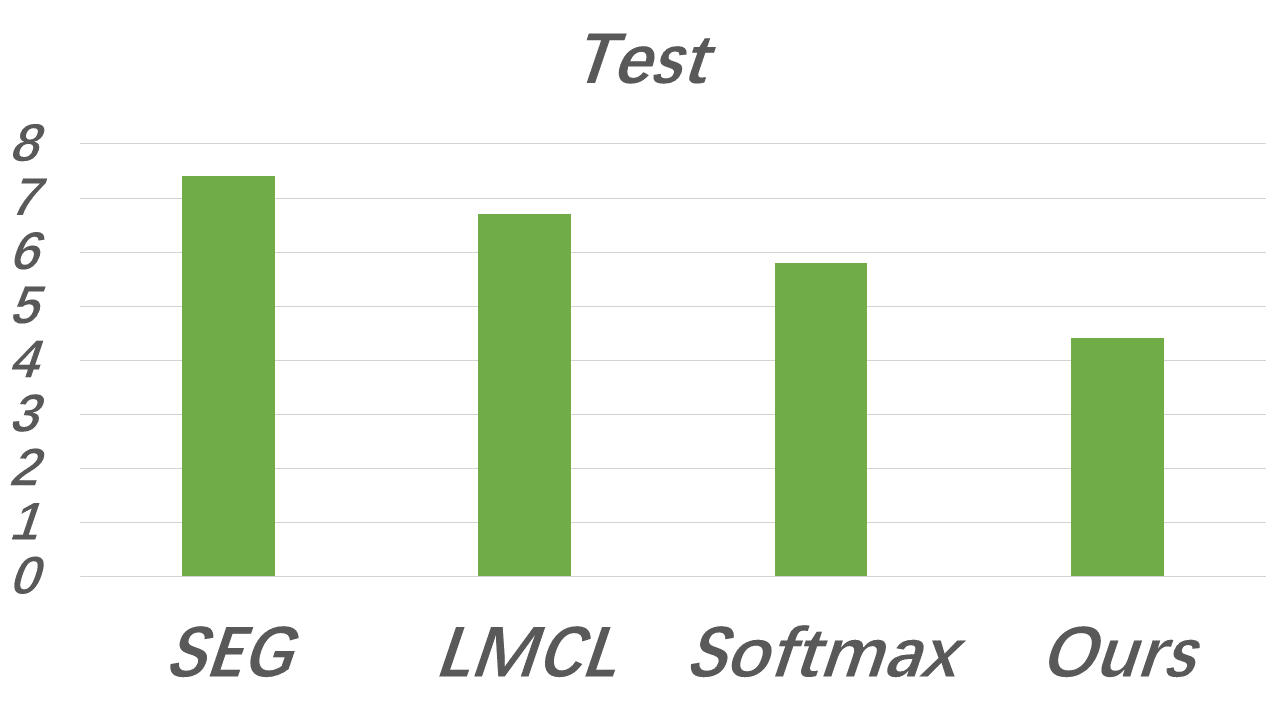
\includegraphics[width=1.\linewidth,height=0.11\textheight]{efficiency_test.png}
%   \caption{Self-Supervised Accuracy}
%   \label{fig:convex_acc}
\end{subfigure}%
\begin{subfigure}{0.23\textwidth}
  \centering
  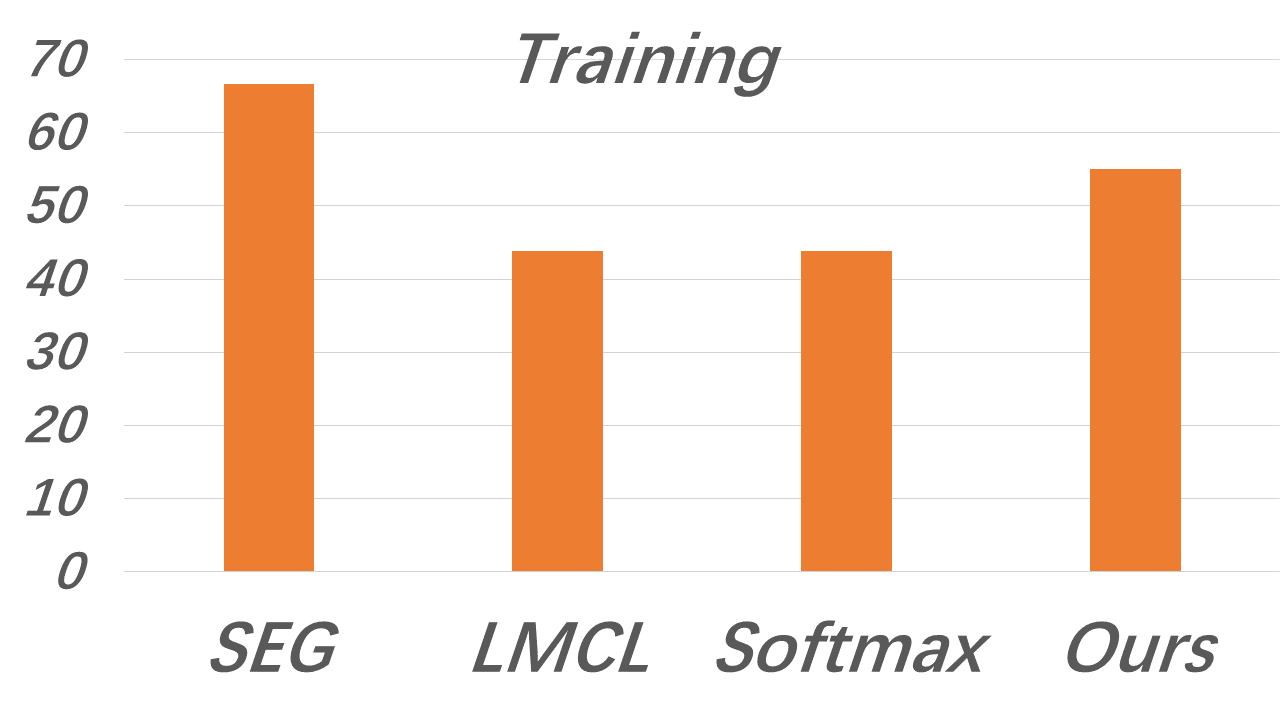
\includegraphics[width=1.\linewidth,height=0.11\textheight]{efficiency_train.png}
%   \caption{Self-Supervised Unknown F1}
%   \label{fig:convex_f1}
\end{subfigure}
\caption{Comparison of training time (per epoch) and test time with baselines.}
\label{fig:efficiency}
\end{figure}


\subsection{Efficiency}
We provide a quantitative comparison on the training and test efficiency for our method and the baselines, by calculating the average time (in seconds) for training per epoch and the total time for testing under the $75\%$ setting. Here, we only compare with the strongest baselines. As shown in Figure~\ref{fig:efficiency}, even with the pseudo outliers, the training time of our method is comparable to that of the baselines. Importantly, in the test stage, our method demonstrates significant advantages in efficiency, which needs much less time to predict intent classes for all samples in the test set.

% \begin{table}
% \centering
% % \setlength{\tabcolsep}{2.0pt}
% \small
% \begin{tabular}{lcccc}
% \hline
% Dataset&CLINK150&StackOverflow&Banking&MICD-EN\\
% \hline
% Vocab Size&8376&17,182&5028&1254\\
% \# Avg. Length&8.31&9.18&11.91&6.74\\
% \# of Samples&23,700&2,000&1,3083&1,745\\
% \hline
% \end{tabular}
% \caption{\label{table:datsets_stats}
% summary of datasets.
% }
% \end{table}



\section{Conclusion}

We have proposed a simple, effective, and efficient approach for out-of-scope intent detection by overcoming the limitation of previous methods via matching train-test conditions. Particularly, at the training stage, we construct self-supervised and open-domain outliers to improve model generalization and simulate real outliers in the test stage. Extensive experiments on four dialogue datasets show that our approach significantly outperforms state-of-the-art methods. In the future, we plan to investigate the theoretical underpinnings of our approach and apply it to more applications.

%for out-of-scope intent detection in different scenarios such as cross-domain and few-shot learning scenarios.
%, and achieves large performance gains especially when the amount of training data is relatively small. I

%forming a consistent $K+1$ classification task for training and test. In particular, we construct \emph{hard} self-supervised outliers and \emph{easy} open-domain outliers at the training stage without utilizing any of information of outlliers in the test set. Extensive experiments demonstrate the effectiveness of our method. Our method results in favorable performance on unknown intent classification and provides especially significant improvement in data-scarce scenarios. In the future, we will study the effect of our propose method in diverse unknown intent classification tasks, such as cross-domain and few-shot scenarios.

\section*{Acknowledgments}

We would like to thank the anonymous reviewers for their helpful comments. This research was supported by the grant HK ITF UIM/377.

% \begin{table}
% \centering
% \begin{tabular}{lrl}
% \hline \textbf{Type of Text} & \textbf{Font Size} & \textbf{Style} \\ \hline
% paper title & 15 pt & bold \\
% author names & 12 pt & bold \\
% author affiliation & 12 pt & \\
% the word ``Abstract'' & 12 pt & bold \\
% section titles & 12 pt & bold \\
% subsection titles & 11 pt & bold \\
% document text & 11 pt  &\\
% captions & 10 pt & \\
% abstract text & 10 pt & \\
% bibliography & 10 pt & \\
% footnotes & 9 pt & \\
% \hline
% \end{tabular}
% \caption{\label{font-table} Font guide. }
% \end{table}







% \begin{table}
% \centering
% \begin{tabular}{lc}
% \hline
% \textbf{Command} & \textbf{Output}\\
% \hline
% \verb|{\"a}| & {\"a} \\
% \verb|{\^e}| & {\^e} \\
% \verb|{\`i}| & {\`i} \\ 
% \verb|{\.I}| & {\.I} \\ 
% \verb|{\o}| & {\o} \\
% \verb|{\'u}| & {\'u}  \\ 
% \verb|{\aa}| & {\aa}  \\\hline
% \end{tabular}
% \begin{tabular}{lc}
% \hline
% \textbf{Command} & \textbf{Output}\\
% \hline
% \verb|{\c c}| & {\c c} \\ 
% \verb|{\u g}| & {\u g} \\ 
% \verb|{\l}| & {\l} \\ 
% \verb|{\~n}| & {\~n} \\ 
% \verb|{\H o}| & {\H o} \\ 
% \verb|{\v r}| & {\v r} \\ 
% \verb|{\ss}| & {\ss} \\
% \hline
% \end{tabular}
% \caption{Example commands for accented characters, to be used in, \emph{e.g.}, \BibTeX\ names.}\label{tab:accents}
% \end{table}



% \begin{table*}
% \centering
% \begin{tabular}{lll}
% \hline
% \textbf{Output} & \textbf{natbib command} & \textbf{Old ACL-style command}\\
% \hline
% \citep{Gusfield:97} & \small\verb|\citep| & \small\verb|\cite| \\
% \citealp{Gusfield:97} & \small\verb|\citealp| & no equivalent \\
% \citet{Gusfield:97} & \small\verb|\citet| & \small\verb|\newcite| \\
% \citeyearpar{Gusfield:97} & \small\verb|\citeyearpar| & \small\verb|\shortcite| \\
% \hline
% \end{tabular}
% \caption{\label{citation-guide}
% Citation commands supported by the style file.
% The style is based on the natbib package and supports all natbib citation commands.
% It also supports commands defined in previous ACL style files for compatibility.
% }
% \end{table*}


% \begin{itemize}
% \item Example article in journal: \citep{Ando2005}.
% \item Example article in proceedings, with location: \citep{borschinger-johnson-2011-particle}.
% \item Example article in proceedings, without location: \citep{andrew2007scalable}.
% \item Example arxiv paper: \citep{rasooli-tetrault-2015}. 
% \end{itemize}




% \section*{Acknowledgments}

% The acknowledgments should go immediately before the references. Do not number the acknowledgments section.
% \textbf{Do not include this section when submitting your paper for review.}

\bibliographystyle{acl_natbib}
\bibliography{anthology,acl2021}

%\appendix



\end{document}
